\begin{name}
	{NGUYÊN HÀM - TÍCH PHÂN}
	{KT NGUYÊN HÀM}
	{\tentruong}
	{\thoigian}
\end{name}
\setcounter{ex}{0}\setcounter{bt}{0}
\Opensolutionfile{ans}[ans/ans-2-B11-De1-lc]
\TN
\begin{ex}%Câu 1%[2D4N1-2]
	Họ nguyên hàm của hàm số $f(x)=x^3$ là
	\choice
	{$4x^4+C$}
	{$3x^2+C$}
	{$x^4+C$}
	{\True $\dfrac{1}{4}x^4+C$}
	\loigiai{
Ta có 
	$\displaystyle\int x^3\mathrm{\,d}x=\dfrac{1}{4}x^4+C$.
}
\end{ex}

\begin{ex}%Câu 2%[2D4N1-3]
	Tìm nguyên hàm của hàm số $ f(x)=2\sin x$.
	\choice
	{\True $\displaystyle\int 2\sin x\mathrm{\,d}x=-2\cos x+C$}
	{$\displaystyle\int 2\sin x\mathrm{\,d}x=2\cos x+C$}
	{$\displaystyle\int 2\sin x\mathrm{\,d}x=\sin^2x+C$}
	{$\displaystyle\int 2\sin x\mathrm{\,d}x=\sin 2x+C$}
	\loigiai{
Ta có $\displaystyle\int 2\sin x\mathrm{\,d}x=2\displaystyle\int \sin x \mathrm{\,d}x=-2\cos x+C$.}
\end{ex}

\begin{ex}%Câu 3%[2D4N1-4]
	Họ nguyên hàm của hàm số $f(x)=\mathrm{e}^x+x$ là
	\choice
	{$\mathrm{e}^x+1+C$}
	{$\mathrm{e}^x+x^2+C$}
	{\True $\mathrm{e}^x+\dfrac{1}{2}{x^2}+C$}
	{$\dfrac{1}{x+1}{\mathrm{e}^x}+\dfrac{1}{2}{x^2}+C$}
	\loigiai{
Ta có $\displaystyle\int \left(\mathrm{e}^x+x\right) \mathrm{\,d}x=\displaystyle\int \mathrm{e}^x \mathrm{\,d}x+\displaystyle\int x \mathrm{\,d}x=\mathrm{e}^x+\dfrac{x^2}{2}+C$.}
\end{ex}

\begin{ex}%Câu 4%[2D4N1-2]
	Họ nguyên hàm của hàm số $y=x^2-3x+\dfrac{1}{x}$ là
	\choice
	{$\dfrac{x^3}{3}-\dfrac{3x^2}{2}-\ln\left|x\right|+C$}
	{$\dfrac{x^3}{3}-\dfrac{3x^2}{2}+\ln x+C$}
	{\True $\dfrac{x^3}{3}-\dfrac{3x^2}{2}+\ln\left|x\right|+C$}
	{$\dfrac{x^3}{3}-\dfrac{3x^2}{2}+\dfrac{1}{x^2}+C$}
	\loigiai{
	Ta có 
		$\displaystyle\int \left(x^2-3x+\dfrac{1}{x}\right) \mathrm{\,d}x=\dfrac{x^3}{3}-\dfrac{3x^2}{2}+\ln\left|x\right|+C$.
	
}
\end{ex}

\begin{ex}%Câu 5%[2D4H1-2]
	Tìm nguyên hàm của hàm số $f(x)=\dfrac{x^4+2}{x^2}$.
	\choice
	{$\displaystyle\int f(x)\mathrm{\,d}x=\dfrac{x^3}{3}-\dfrac{1}{x}+C$}
	{$\displaystyle\int f(x)\mathrm{\,d}x=\dfrac{x^3}{3}+\dfrac{2}{x}+C$}
	{$\displaystyle\int f(x)\mathrm{\,d}x=\dfrac{x^3}{3}+\dfrac{1}{x}+C$}
	{\True $\displaystyle\int f(x)\mathrm{\,d}x=\dfrac{x^3}{3}-\dfrac{2}{x}+C$}
	\loigiai{
Ta có
		$\displaystyle\int \dfrac{x^4+2}{x^2} \mathrm{\,d}x=\displaystyle\int \left(x^2+\dfrac{2}{x^2}\right) \mathrm{\,d}x=\dfrac{x^3}{3}-\dfrac{2}{x}+C$.}
\end{ex}

\begin{ex}%Câu 6%[2D4N1-3]
	Cho hàm số $ f(x)=1-\dfrac{1}{\cos^2 x}$. Khẳng định nào dưới đây đúng?
	\choice
	{$\displaystyle\int f(x)\mathrm{\,d}x=x+\tan x+C$}
	{$\displaystyle\int f(x)\mathrm{\,d}x=x+\cot x+C$}
	{\True $\displaystyle\int f(x)\mathrm{\,d}x=x-\tan x+C$}
	{$\displaystyle\int f(x)\mathrm{\,d}x=x-\cot x+C$}
	\loigiai{
Ta có $\displaystyle\int f(x) \mathrm{\,d}x=\displaystyle\int \left(1-\dfrac{1}{\cos^2x}\right)\mathrm{\,d}x=\displaystyle\int  \mathrm{\,d}x-\displaystyle\int \dfrac{\mathrm{\,d}x}{\cos^2x}=x-\tan x+C$.}
\end{ex}

\begin{ex}%Câu 7%[2D4N1-3]
	Họ nguyên hàm của hàm số $f(x)=\cos x+6x$ là
	\choice
	{\True $\sin x+3x^2+C$}
	{$-\sin x+3x^2+C$}
	{$\sin x+6x^2+C$}
	{$-\sin x+C$}
	\loigiai{
Ta có $\displaystyle\int f(x)\mathrm{\,d}x=\displaystyle\int \left(\cos x+6x\right)\mathrm{\,d}x=\sin x+3x^2+C$.}
\end{ex}

\begin{ex}%Câu 8%[2D4N1-2]
	$\displaystyle\int f(x)\mathrm{\,d}x=4x^3+x^2+C$ thì hàm số $f(x)$ bằng
	\choice
	{$f(x)=x^4+\dfrac{x^3}{3}+Cx$}
	{$f(x)=12x^2+2x+C$}
	{\True $f(x)=12x^2+2x$}
	{$f(x)=x^4+\dfrac{x^3}{3}$}
	\loigiai{
		Ta có $ f(x)=F'(x)=\left(4x^3+x^2+C\right)'=12x^2+2x$.}
\end{ex}

\begin{ex}%Câu 9%[2D4N1-4]
	Hàm số $F(x)=2x+3^x-1$ là nguyên hàm của hàm số nào trong các hàm số sau
	\choice
	{\True $f(x)=2+3^x\ln 3$}
	{$f(x)=x^2+\dfrac{3^x}{\ln 3}-x+C$}
	{$f(x)=x^2+\dfrac{3^x}{\ln 3}-x$}
	{$f(x)=2+3^x\ln 3+C$}
	\loigiai{
	Ta có $ f(x)=F'(x)\Rightarrow f(x)=\left(2x+3^x-1\right)'=2+3^x\ln 3$.}
\end{ex}

\begin{ex}%Câu 10%[2D4H1-4]
	Cho$\displaystyle\int \ln x \mathrm{\,d}x=F(x)+C$. Khẳng định nào dưới đây đúng?
	\choice
	{$F'(x)=\dfrac{1}{x}$}
	{$F'(x)=\dfrac{1}{x}+C$} 
	{\True $F'(x)=\ln x$}
	{$F'(x)=\ln x+1$}
	\loigiai{
Ta có $ F'(x)=f(x)=\ln x$.}
\end{ex}

\begin{ex}%Câu 11%[2D4H1-4]
	Cho $F(x)$ là một nguyên hàm của hàm số $f(x)=\mathrm{e}^x+2x$ thỏa mãn $F(0)=\dfrac{3}{2}$. Tìm $F(x)$.
	\choice
	{\True $F(x)=\mathrm{e}^x+x^2+\dfrac{1}{2}$}
	{$F(x)=\mathrm{e}^x+x^2+\dfrac{5}{2}$}
	{$F(x)=\mathrm{e}^x+x^2+\dfrac{3}{2}$}
	{$F(x)=2\mathrm{e}^x+x^2-\dfrac{1}{2}$}
	\loigiai{
Ta có $ F(x)=\displaystyle\int\left(\mathrm{e}^x+2x\right) \mathrm{\,d}x=e^x+x^2+C$.\\
		Theo bài ra ta có $F(0)=1+C=\dfrac{3}{2}\Rightarrow C=\dfrac{1}{2}$.}
\end{ex}

\begin{ex}%Câu 12%[2D4H1-6]
	Một viên đạn được bắn thẳng đứng lên trên từ mặt đất. Giả sử tại thời điểm $t$ giây (coi $t=0$ là thời điểm viên đạn được bắn lên), vận tốc của nó được cho bởi $v(t)=160-9{,}8t$ (m/s). Độ cao của viên đạn (tính từ mặt đất) sau $t=10$ giây là
	\choice
	{$620$ m}
	{$1\,240$ m}
	{$555$ m}
	{\True $1\,110$ m}
	\loigiai{
Gọi $S(t)$ là độ cao của viên đạn sau $t$ giây kể từ lúc bắt đầu bắn.\\
		Ta có $v(t)=S'(t)$. Do đó, $S(t)$ là một nguyên hàm của vận tốc $ v(t)$.\\
		$S(t)=\displaystyle\int v(t) \mathrm{\,d}t=\displaystyle\int \left(160-9{,}8t\right)\mathrm{\,d}t=160t-4{,}9t^2+C$.\\
		Theo giả thiết, $S(0)=0$ nên $C=0$ và ta được $S(t)=160t-4{,}9t^2$ (m).\\
		Độ cao của viên đạn sau $t=10$ giây là
		$S(10)=160\cdot 10-4{,}9\cdot10^2=1\,110$ (m).\\
		Vậy độ cao của viên đạn (tính từ mặt đất) sau $t=10$ giây là $ 1\,110$ (m).\\
}
\end{ex}
 \Closesolutionfile{ans}
\indapan{6}{ans/ans-2-B11-De1-lc}
\Opensolutionfile{ans}[ans/ans-2-B11-De1-ds]
\TNTF
\begin{ex}%Câu 13%[2D4H1-4]
	Cho hàm số $y=h(x)$ có đạo hàm $h'(x)=3x^2$ và hàm số $y=g(x)$ có đạo hàm $g'(x)=\mathrm{e}^x$.
	\choiceTF
	{Hàm số $y=h(x)=6x+C_1$, với $C_1\in \mathbb{R}$}
	{\True Hàm số $y=g(x)=\mathrm{e}^x+C_2$, với $C_2\in \mathbb{R}$}
	{\True $ I=\displaystyle\int \left[xh'(x)+2025\right]\mathrm{\,d}x=\dfrac{3}{4}{x^4}+2025x+C$ với $C\in \mathbb{R}$}
	{\True Cho $ f'(x)=3x^2+\mathrm{e}^x+m-1$. Cho $f(0)=2$; $ f(1)=2\mathrm{e}$ thì giá trị của $m\in (1;2)$}
\loigiai{
\begin{itemchoice}
	\itemch \textbf{Sai}. Ta có $ h(x)=\displaystyle\int h'(x) \mathrm{\,d}x=3\displaystyle\int x^2\mathrm{\,d}x=x^3+C_1$.
	\itemch \textbf{Đúng}. Ta có $ g(x)=\displaystyle\int g'(x)\mathrm{\,d}x=\displaystyle\int \mathrm{e}^x\mathrm{\,d}x=\mathrm{e}^x+C_2$.
	\itemch \textbf{Đúng}. Ta có $ I=\displaystyle\int \left[xh'(x)+2025\right]\mathrm{\,d}x=\displaystyle\int \left[3x^3+2025\right]\mathrm{\,d}x=\dfrac{3}{4}{x^4}+2025x+C$.
	\itemch \textbf{Đúng}. Ta có $ f(x)=\displaystyle\int f'(x)\mathrm{\,d}x=\displaystyle\int \left(3x^2+\mathrm{e}^x+m-1\right)\mathrm{\,d}x=x^3+\mathrm{e}^x+(m-1)x+C$.\\
	Vì $\heva{
		&f(0)=2\\
		&f(1)=2\mathrm{e}}
	\Rightarrow\heva{
		&1+C=2\\
		&1+\mathrm{e}+m-1+C=2\mathrm{e}}
\Rightarrow\heva{
		&C=1\\
		&m=\mathrm{e}-1.}
	$\\
	Vậy $m=\mathrm{e}-1\Rightarrow 1<m<2$.
	\end{itemchoice}
}
\end{ex}

\begin{ex}%Câu 14%[2D4H1-3]
Cho các hàm số $g(x)=\sin x$ , $h(x)=\cos x$.
\choiceTF
{$\displaystyle\int \left[2g(x)-3h(x)\right]\mathrm{\,d}x=3\displaystyle\int g(x)\mathrm{\,d}x-2\displaystyle\int h(x)\mathrm{\,d}x$}
{\True Một nguyên của hàm số $g(x)$ là $-\cos x$}
{Họ nguyên của hàm số $h(x)+2\sqrt{x}$ là $\sin x+\dfrac{3}{2}\sqrt{x^3}+C$}
{\True Họ nguyên hàm của hàm số $f(x)=g(x)\cdot h^2(x)$ là $F(x)=-\dfrac{1}{3}\cos^3 x+C$}
\loigiai{
\begin{itemchoice}
\itemch \textbf{Sai}. Ta có $\displaystyle\int \left[2g(x)-3h(x)\right]\mathrm{\,d}x=2\displaystyle\int g(x)\mathrm{\,d}x-3\displaystyle\int h(x)\mathrm{\,d}x$.
\itemch \textbf{Đúng}. Ta có $\displaystyle\int g(x)\mathrm{\,d}x=\displaystyle\int \sin x \mathrm{\,d}x=-\cos x+C$ nên một nguyên của hàm số $g(x)$ là $-\cos x$.
\itemch \textbf{Sai}. Ta có $\displaystyle\int \left[h(x)+2\sqrt x\right]\mathrm{\,d}x=\displaystyle\int \cos x\mathrm{\,d}x+2\displaystyle\int x^{\tfrac{1}{2}}\mathrm{\,d}x=\sin x+\dfrac{4}{3}\sqrt{x^3}+C$.
\itemch \textbf{Đúng}. Ta có $F'(x)=-\cos^2 x\cdot (\cos x)'=-\cos ^2 x\cdot (-\sin x)=\sin x\cdot \cos^2 x=g(x)\cdot h^2(x)$.
\end{itemchoice}}
\end{ex} 
\begin{ex}%Câu 15%[2D4H1-4]
Cho các hàm số $g(x)=\dfrac{1}{x^2}$, $h(x)=\ln (x+3)$.
\choiceTF
{ Biết $G(x)$ là một nguyên hàm của $g(x)$ và $ G(1)=1$. Khi đó $ G(2)=-\dfrac{1}{2}$}
{\True $ J=\displaystyle\int \left[h(x)+\ln\dfrac{1}{x+3}+2025\right]\mathrm{\,d}x=2025x+C$}
{$I=\displaystyle\int x\cdot h'(x)\mathrm{\,d}x=x-\ln (x+3)+C$ với $C\in \mathbb{R}$}
{\True Giả sử $F(x)$ là một nguyên hàm của $f(x)=\dfrac{x+3}{g(x)}$ và $F(1)=\dfrac{1}{4}$.\\ Khi đó $F(-1)=-\dfrac{7}{4}$}
\loigiai{
\begin{itemchoice}
\itemch \textbf{Sai}. Ta có $ G(x)=\displaystyle\int{g(x)}{\rm{d}}x=\displaystyle\int{\dfrac{1}{x^2}}{\rm{d}}x=\displaystyle\int{x^{-2}}{\rm{d}}x=-\dfrac{1}{x}+C$.\\
Mà $ G(1)=1\Rightarrow C=2$ $\Rightarrow G(x)=-\dfrac{1}{x}+2\Rightarrow G(2)=\dfrac{3}{2}$.
\itemch \textbf{Đúng}. Ta có 
\begin{eqnarray*}
 J&=&\displaystyle\int \left[h(x)+\ln\dfrac{1}{x+3}+2025\right]\mathrm{\,d}x=2025x+C\\
&=&\displaystyle\int \left[\ln (x+3) + \ln\dfrac{1}{x+3}+2025 \right]\mathrm{\,d}x\\
&=&\displaystyle\int \left(\ln 1+2025\right)\mathrm{\,d}x=2025x+C.
\end{eqnarray*}
\itemch \textbf{Sai}. Ta có $\left[x-\ln\left(x+3\right)+C\right]'=1-\dfrac{1}{x+3}=\dfrac{x+2}{x+3}. \quad(1)$ \\
Và $ x\cdot h'(x)=x\cdot \left(\ln (x+3)\right)'=\dfrac{x}{x+3}. \quad(2)$\\
Từ $(1)$ và $(2)$ suy ra $\displaystyle\int xh'(x)\mathrm{\,d}x \ne x-\ln (x+3)+C$.\\
\itemch \textbf{Đúng}. Ta có 
\begin{eqnarray*}
	\displaystyle\int \dfrac{x+3}{g(x)}\mathrm{\,d}x &=&\displaystyle\int \dfrac{x+3}{\dfrac{1}{x^2}}\mathrm{\,d}x\\
	&=&\displaystyle\int x^2(x+3)\mathrm{\,d}x=\displaystyle\int x^3\mathrm{\,d}x+3\displaystyle\int x^2\mathrm{\,d}x\\
	&=&\dfrac{1}{4}{x^4}+x^3+C.
\end{eqnarray*}
Mà $F(1)=\dfrac{1}{4}\Leftrightarrow C=-1$.\\
$F(x)=\dfrac{1}{4}{x^4}+x^3-1\Rightarrow F(-1)=-\dfrac{7}{4}$.
\end{itemchoice}
}
\end{ex}
\begin{ex}%Câu 16%[2D4H1-4]
Cho các hàm số $g(x)=\mathrm{e}^{\tfrac{x}{2}}$, $h(x)=2x^3+5x^2-2x+4$.
\choiceTF
{\True $\displaystyle\int \left[2g(x)+3h(x)\right]\mathrm{\,d}x=2\displaystyle\int g(x)\mathrm{\,d}x+3\displaystyle\int h(x)\mathrm{\,d}x$}
{\True Một nguyên của hàm số $3\cdot g^2(x)$ là $3\mathrm{e}^x$}
{Họ nguyên của hàm số $h(x)$ là $\dfrac{1}{4}{x^3}+\dfrac{5}{3}{x^3}-x^2+C$}
{\True Biết $\displaystyle\int g^4(x)\cdot h(x)\mathrm{\,d}x=(a{x^3}+b{x^2}+cx+d)\mathrm{e}^{2x}+C$. Khi đó $ a+b+c+d=3$}
\loigiai{
\begin{itemchoice}
\itemch \textbf{Đúng}. Ta có $\displaystyle\int \left[2g(x)+3h(x)\right]\mathrm{\,d}x=2\displaystyle\int g(x)\mathrm{\,d}x+3\displaystyle\int h(x)\mathrm{\,d}x$.
\itemch \textbf{Đúng}. Ta có $\displaystyle\int 3g^2(x)=3\displaystyle\int \mathrm{e}^x\mathrm{\,d}x=3\mathrm{e}^x+C$.
\itemch \textbf{Sai}. Ta có $\displaystyle\int h(x)\mathrm{\,d}x=\displaystyle\int \left(2x^3+5x^2-2x+4\right)\mathrm{\,d}x=\dfrac{1}{2}{x^4}+\dfrac{5}{3}{x^3}-x^2+4x+C$.
\itemch \textbf{Đúng}. Ta có 
\begin{eqnarray*}
	&&\displaystyle\int g^4(x)\cdot h(x)\mathrm{\,d}x=(a{x^3}+b{x^2}+cx+d){\mathrm{e}^{2x}}+C\\
	&\Leftrightarrow& \displaystyle\int{\mathrm{e}^{2x}}(2x^3+5x^2-2x+4)\mathrm{\,d}x=(a{x^3}+b{x^2}+cx+d){\mathrm{e}^{2x}}+C.
\end{eqnarray*}
Nên
\begin{eqnarray*}
	\left((ax^3+bx^2+cx+d)\mathrm{e}^{2x}+C\right)'&=&(3ax^2+2bx+c)\mathrm{e}^{2x}+2\mathrm{e}^{2x}\left(ax^3+bx^2+cx+d\right)\\
	&=&\left(2ax^3+(3a+2b)x^2+(2b+2c)x+c+2d\right)\mathrm{e}^{2x}\\
	&=&(2x^3+5x^2-2x+4)\mathrm{e}^{2x}.
\end{eqnarray*}
Do đó $\heva{&2a=2\\&3a+2b=5\\&2b+2c=-2\\
&c+2d=4}\Leftrightarrow\heva{&a=1\\&b=1\\&c=-2\\&d=3.}$\\
Vậy $a+b+c+d=3$.
\end{itemchoice}
}
\end{ex}
\Closesolutionfile{ans}
\indapan{2}{ans/ans-2-B11-De1-ds}
\Opensolutionfile{ans}[ans/ans-2-B11-De1-kq]
\TNSA
\begin{ex}%Câu 17%[2D4H1-3]
Cho $F(x)$ là một nguyên hàm của hàm $f(x)=\dfrac{\cos 2x}{\sin x+\cos x}$ thỏa mãn $F(0)=1$. Tính $F(\pi)$.
\shortans{-1}
\loigiai{
Ta có
\allowdisplaybreaks
\begin{eqnarray*}
	F(x)&=&\displaystyle\int \dfrac{\cos 2x}{\sin x+\cos x}\mathrm{\,d}x 
	=\displaystyle\int \dfrac{\cos^2x-\sin^2x}{\sin x+\cos x}\mathrm{\,d}x\\
	&=&\displaystyle\int \dfrac{(\sin x+\cos x)(\cos x-\sin x)}{\sin x+\cos x} \mathrm{\,d}x\\
	&=&\displaystyle\int (\cos x-\sin x)\mathrm{\,d}x=\sin x+\cos x+C.
\end{eqnarray*}
Do $F(0)=1$ nên $C=0\Rightarrow F(x)=\sin x+\cos x \Rightarrow F(\pi)=-1$.}
\end{ex}

\begin{ex}%Câu 18%[2D4V1-4]
$F(x)$ là một nguyên hàm của hàm số $f(x)=2^x$, thỏa mãn $ F(0)=\dfrac{1}{\ln 2}$. Biểu thức $ F(0)+F(1)+F(2)+\ldots+F(2024)=\dfrac{a^b-c}{\ln a}$ $(a$, $b$, $c\in{N^*})$. Tính $ T=a+b-2c$.
\shortans{2025}
\loigiai{
Ta có $F(x)=\displaystyle\int 2^x \mathrm{\,d}x=\dfrac{2^x}{\ln 2}+C$.\\
Theo giả thiết $F(0)=\dfrac{1}{\ln 2}\Leftrightarrow\dfrac{2^0}{\ln 2}+C=\dfrac{1}{\ln 2}\Leftrightarrow C=0 \Rightarrow F(x)=\dfrac{2^x}{\ln 2}$.\\
Khi đó 
\allowdisplaybreaks
\begin{eqnarray*}
	F(0)+F(1)+F(2)+\ldots+F(2024)&=&\dfrac{2^0}{\ln 2}+\dfrac{2^1}{\ln 2}+\dfrac{2^2}{\ln 2}+\ldots+\dfrac{2^{2024}}{\ln 2}\\
	&=&\dfrac{1}{\ln 2}(2^0+2^1+2^2+\ldots+2^{2024})\\
	&=&\dfrac{1}{\ln 2}\cdot \dfrac{1(1-2^{2025})}{1-2}=\dfrac{2^{2025}-1}{\ln 2}.
\end{eqnarray*}
$\Rightarrow a=2$, $b=2025$, $c=1$.\\
Vậy $ T=a+b-2c=2025$.}
\end{ex}

\begin{ex}%Câu 19%[2D4V1-2]
Gọi $F(x)$ là một nguyên hàm của hàm số $f(x)=\dfrac{(3x-1)^2}{x^2}$, biết đồ thị hàm số $y=F(x)$ đi qua điểm $M(1;-2)$. Tính $F\left(\mathrm{e}^2\right)$ (làm tròn kết quả đến hàng phần chục).
\shortans{44{,}4}
\loigiai{
Ta có
\allowdisplaybreaks
\begin{eqnarray*}
F(x)&=&\displaystyle\int \dfrac{(3x-1)^2}{x^2}\mathrm{\,d}x=\displaystyle\int \left(\dfrac{9x^2-6x+1}{x^2}\right) \mathrm{\,d}x\\
&=&\displaystyle\int \left(9-\dfrac{6}{x}+\dfrac{1}{x^2}\right) \mathrm{\,d}x\\
&=&9\displaystyle\int \mathrm{\,d}x-6\displaystyle\int\dfrac{1}{x} \mathrm{\,d}x+\displaystyle\int x^{-2} \mathrm{\,d}x\\
&=&9x-6\ln\left| x\right|-\dfrac{1}{x}+C.
\end{eqnarray*}
Theo giả thiết, đồ thị hàm số $y=F(x)$ đi qua điểm $M(1;-2)$ nên suy ra
\allowdisplaybreaks
\begin{eqnarray*}
F(1)=-2&\Rightarrow &9-6\ln 1-1+C=-2\\
&\Rightarrow & C=-10\Rightarrow F(x)=9x-6\ln\left|x\right|-\dfrac{1}{x}-10\\
&\Rightarrow& F\left(e^2\right)=9e^2-6\ln\left|\mathrm{e}^2\right|-\dfrac{1}{\mathrm{e}^2}-10\approx 44{,}4.
\end{eqnarray*}
}
\end{ex}

\begin{ex}%Câu 20%[2D4V1-6]
Một xe ô tô đang chạy với tốc độ $90$ km/h thì người lái xe bất ngờ phát hiện chướng ngại vật trên đường cách đó $150$ m. Người lái xe phản ứng $2$ giây sau đó bằng cách đạp phanh cho xe chạy chậm hơn. Kể từ thời điểm này, ô tô chuyển động chậm dần đều với tốc độ $v(t)=-\dfrac{25}{4}t+25$(m/s), trong đó $t$ là thời gian tính bằng giây kể từ lúc đạp phanh. Quãng đường xe ô tô đã di chuyển kể từ lúc người lái xe phát hiện chướng ngại vật trên đường đến khi xe ô tô dừng hẳn là bao nhiêu mét?\\
\shortans{100}
\loigiai{
Gọi $s(t)$ là quãng đường xe ô tô đi được trong $t$ (giây) kể từ lúc đạp phanh.\\ Khi đó
$ s(t)=\displaystyle\int v(t) \mathrm{\,d}t=\displaystyle\int \left(-\dfrac{25}{4}t+25\right) \mathrm{\,d}t=-\dfrac{25}{8}{t^2}+25t+C$.\\
Do $s(0)=0$ nên $C=0$ . Suy ra $s(t)=-\dfrac{25}{8}{t^2}+25t$.\\
Xe ô tô dừng hẳn khi $ v(t)=0\Leftrightarrow-\dfrac{25}{4}t+25=0\Leftrightarrow t=4$.\\
Suy ra quãng đường xe ô tô còn di chuyển được kể từ lúc đạp phanh đến khi xe dừng hẳn là 
$s(4)=-\dfrac{25}{8}{4^2}+25\cdot 4=50$ (m).\\
Ta có tốc độ $90$ km/h cũng là tốc độ $25$ m/s.\\
Do đó, quãng đường xe ô tô đã di chuyển kể từ lúc người lái xe phát hiện chướng ngại vật trên đường đến khi xe ô tô dừng hẳn là: $ 25\cdot 2+50=100$ (m).
}
\end{ex}

\begin{ex}%Câu 21%[2D4V1-6]
Một quần thể vi khuẩn ban đầu gồm $500$ vi khuẩn, sau đó bắt đầu tăng trưởng. Gọi $P(t)$ là số lượng vi khuẩn của quần thể đó tại thời điểm $t$, trong đó $ t$ tính theo ngày $(0\le t\le 10)$. Tốc độ tăng trưởng của quần thể vi khuẩn đó cho bởi hàm số $P'(t)=k\sqrt{t}$, trong đó k là hằng số. Sau 1 ngày, số lượng vi khuẩn của quần thể đó đã tăng lên thành 600 vi khuẩn (Nguồn: R. Larson and
Edwards, Calculus 10e, Cengage 2014). Tính số lượng vi khuẩn của quần thể đó sau $9$ ngày.

\shortans{3200}
\loigiai{
Ta có $P(t)=\displaystyle\int P'(t)\mathrm{\,d}t=\displaystyle\int k\sqrt{t} \mathrm{\,d}t=\displaystyle\int k\cdot t^{\tfrac{1}{2}}\mathrm{\,d}t=k\cdot\dfrac{2}{3}t\sqrt{t}+C$.\\
Từ giả thiết suy ra $\heva{&P(0)=500\\&P(1)=600
}\Rightarrow\heva{&k\cdot\dfrac{2}{3}\cdot0\sqrt 0+C=500\\&k\cdot\dfrac{2}{3}\cdot1\sqrt 1+C=600}\Rightarrow\heva{&C=500\\&
\dfrac{2}{3}k=100}\Rightarrow\heva{&C=500\\&k=150.}$\\
$\Rightarrow P(t)=100t\sqrt t+500$.\\
Do đó, số lượng vi khuẩn của quần thể đó sau $9$ ngày là $P(9)=100\cdot 9\sqrt{9}+500=3\,200$.}
\end{ex}

\begin{ex}%Câu 22%[2D4V1-6]
Cây cà chua khi trồng có chiều cao $5$ cm. Tốc độ tăng chiều cao của cây cà chua sau khi trồng được cho bởi hàm số $ v(t)=-0{,}1t^3+t^2$, trong đó $t$ tính theo tuần, $v(t)$ tính bằng cm/tuần. Gọi $h(t)$ (tính bằng centimét) là độ cao của cây cà chua ở tuần thứ $t$ (Nguồn:A. Bigalke et al., Mathematik, Grundkurs ma-I, Cornelsen 2016). Vào thời điểm cây cà chua đó phát triển nhanh nhất thì cây cà chua sẽ cao bao nhiêu? (làm tròn kết quả đến hàng phần chục).
\shortans{54{,}4}
\loigiai{
Ta có $h(t)=\displaystyle\int v(t) \mathrm{\,d}t=\displaystyle\int \left(-0{,}1t^3+t^2\right) \mathrm{\,d}t=-\dfrac{1}{40}{t^4}+\dfrac{t^3}{3}+C$.\\
Cây cà chua khi trồng có chiều cao $5$ cm nên $h(0)=5\Rightarrow C=5$.\\
Vậy độ cao của cây cà chua ở tuần thứ $t$ được cho bởi hàm số\\ 
\centerline {$h(t)=-\dfrac{1}{40}{t^4}+\dfrac{t^3}{3}+5$ $(t\ge 0)$.}\\
Ta tìm $ t$ $(t\ge 0)$ sao cho $v(t)$ đạt giá trị lớn nhất.\\
$v'(t)=-0{,}3t^2+2t$; $ v'(t)=0\Leftrightarrow-0{,}3t^2+2t=0\Leftrightarrow\hoac{&t=0\\&t=\dfrac{20}{3}.}$\\
Bảng biến thiên
\begin{center}
	\begin{tikzpicture}
	\tkzTabInit[espcl=2.5,lgt=1.5,nocadre]
	{$x$/0.7,$y'$/0.7,$y$/2.1}
	{$-\infty$,$0$,$\tfrac{20}{3}$,$+\infty$}
	\tkzTabLine{,-,0,+,0,-,}
	\tkzTabVar{+/$+\infty$,-/$0$,+/$\dfrac{400}{27}$,-/$-\infty$}
\end{tikzpicture}
\end{center}
Từ đó ta thấy $v(t)$ đạt giá trị lớn nhất tại $t=\dfrac{20}{3}$.\\
Khi đó, cây cà chua sẽ đạt chiều cao là $h\left(\dfrac{20}{3}\right)=\dfrac{4\,405}{81}\approx 54{,}4$ (cm).
}
\end{ex}
\Closesolutionfile{ans}
\indapan{6}{ans/ans-2-B11-De1-kq}